% !TEX root = task-3-3-6.tex
% Editable task bank. Append new BankTask blocks at the end of the document.
\documentclass[12pt,a4paper]{article}
\usepackage{physics-textbook}
\usepackage{graphicx,needspace}
\usetikzlibrary{decorations.pathmorphing}
\newif\ifShowSolutions
\ifdefined\TutorEdition
  \ShowSolutionstrue
\else
  \ShowSolutionsfalse % Change to \ShowSolutionstrue to display solutions.
\fi
\newcounter{banktask}
\newsavebox{\BankTaskBox}
\newcommand{\BankTaskContent}[3]{%
  \noindent\textbf{\thebanktask.}\quad #2\par
  \ifShowSolutions
    \Needspace{50mm}% Keep the solution heading with its opening text or diagram.
    #3\par
    \ifdefined\TutorEdition
      \ifcsname TutorSource#1\endcsname
        \nopagebreak\smallskip{\small\csname TutorSource#1\endcsname\par}%
      \fi
    \fi
  \fi
}
\newcommand{\BankTask}[3]{%
  \refstepcounter{banktask}\par\medskip
  \sbox{\BankTaskBox}{\begin{minipage}{\linewidth}%
    \BankTaskContent{#1}{#2}{#3}\end{minipage}}%
  \ifdim\dimexpr\ht\BankTaskBox+\dp\BankTaskBox\relax>\dimexpr\textheight-20mm\relax
    \Needspace{35mm}\BankTaskContent{#1}{#2}{#3}%
  \else
    \Needspace{\dimexpr\ht\BankTaskBox+\dp\BankTaskBox\relax}%
    \noindent\usebox{\BankTaskBox}\par
  \fi
  \medskip
}
\begin{document}
\BookSubsection{3.3.6}{Линии напряжённости электрического поля}


% Source 29998: https://phys-ege.sdamgia.ru/problem?id=29998
\BankTask{29998}{
\begin{center}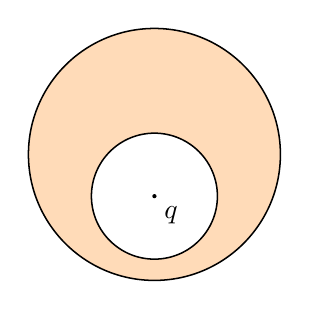
\begin{tikzpicture}[>=stealth,line width=.55pt]\draw[fill=orange!28](0,0)circle(1.6);\draw[fill=white](0,-.53)circle(.8);\fill(0,-.53)circle(.027)node[below right]{$q$};\end{tikzpicture}\end{center}В нижней половине незаряженного металлического шара располагается крупная шарообразная полость, заполненная воздухом. Шар находится в воздухе вдали от других предметов. В центр полости помещен положительный точечный заряд q > $0$ (см. рисунок). Нарисуйте картину линий напряженности электростатического поля внутри полости, внутри проводника и снаружи шара. Если поле отсутствует, напишите в данной области: $\vec{E} = 0.$ Если поле отлично от нуля, нарисуйте картину поля в данной области, используя восемь линий напряженности. Ответ поясните, указав, какие физические закономерности Вы использовали для объяснения.
}{
\smallskip\noindent\textbf{Решение}\par
\begin{center}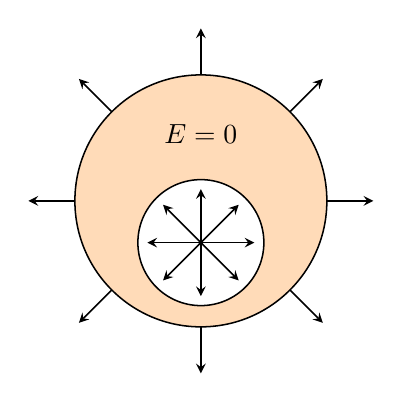
\begin{tikzpicture}[>=stealth,line width=.55pt]\draw[fill=orange!28](0,0)circle(1.6);\draw[fill=white](0,-.53)circle(.8);\node at(0,.85){$E=0$};\foreach \a in {0,45,...,315}{\draw[->](\a:1.6)--(\a:2.19);\draw[->](0,-.53)--++(\a:.68);}\fill(0,-.53)circle(.03);\end{tikzpicture}\end{center}$1$.  Приведен схематический рисунок картины линий напряженности: внутри полости  — семейство прямых лучей, исходящих из заряда и приходящих на поверхность полости по нормали; снаружи шара  — семейство прямых лучей, по нормали к ней и уходящих в бесконечность. 
$2$.  Внутри проводника  — электростатическое поле $\vec{E}=0.$ 
$3$.  Заряд q помещен в центр шарообразной полости, поэтому его электростатическое поле в полости обладает центральной симметрией и выглядит как поле уединенного точечного заряда $q > 0,$ находящегося в центре полости. Линии напряженности этого поля подходят по нормали к поверхности полости, где равномерно распределен отрицательный индуцированный заряд $- q < 0.$ 
$4$.  На наружной поверхности шара находится (в силу нейтральности шара в целом) положительный заряд $q > 0.$ Поскольку внутри проводника $\vec{E}=0,$ а снаружи окружающие предметы расположены далеко от шара, этот заряд распределен по поверхности шара равномерно. Его поле вне шара выглядит как поле уединенного точечного заряда q > $0$, расположенного в центре шара. Линии напряженности отходят от шара по нормали к его поверхности.
}

\end{document}
